In \autoref{chapter:related-work}, the literature review showed that both no-reference image quality analysis and image fusion were addressed by many known techniques such as multiresolution analysis and principal component analysis; on the other hand, applications still evolve as new strategies such as machine learning are presented. The idea that motivated the use of the Fourier Transform as the basis for an IQA method is that it is a fast, robust and reliable analysis tool and could produce relevant results if properly explored. Similarly, the image fusion process was developed by exploring many state-of-the-art fusion applications and addressing both computational requirements (both hardware and software) and computational performance, since the method is built to work on normal optical microscope workstations instead of large clusters. As a result, we studied the capabilities of the Laplacian of Gaussian as the basis for our image fusion algorithm. 

This chapter presents all the details about our no-reference image quality assessment method and our multifocus image fusion method, as well as relevant information about the proposed datasets, including acquisition details and issues. We also show how the methods relate to each other since it also requires the human knowledge to select the images for registration and posterior fusion, similar to most of the z-stacking systems on microscopy software packages.

\section{Overview}
Our approach consists of three parts: a) an image acquisition process based on the z-stacking technique; b) a method for assessing the quality of images that explores frequency domain features and basic statistical analysis tools and outputs a quantitative index that allows the selection of focused images and c) an image fusion procedure, based on the Laplacian of Gaussian filter and energy of edges, which forms the final image. Figure~\ref{fig:overview} graphically summarizes the processing steps, which will be describe in this Chapter. Figure~\ref{fig:overview}.(a) denotes the image acquisition process, which consists of collecting specimens of plants, acquiring images with microscopes and organizing the datasets. Then the images undergo our IQA method in Figure~\ref{fig:overview}.(b), and a subset of the images is selected for registration by means of statistical methods. Finally, Figure~\ref{fig:overview}.(c) represents the image fusion procedure, which aims to produce a high-quality image.

\begin{figure}[ht]
  \centering
  \caption{Overview of each stage of our approach: \textbf{(a)} image acquisition and registration, \textbf{(b)} selection of images after IQA and \textbf{(c)} image fusion.}
  \label{fig:overview}
  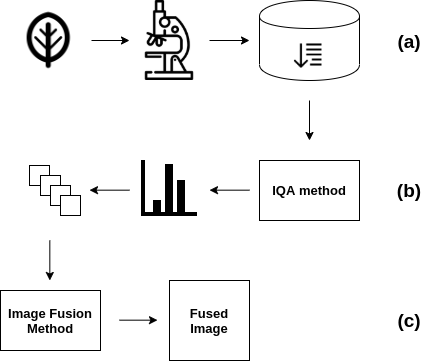
\includegraphics[scale=0.8]{images/overview.png}
  \centering
  \fautor
\end{figure}

\section{Image Datasets}
\section{Proposed dataset}

Three bright-field microscopy images datasets were acquired with the ZEISS Axiocam ERc5s camera in the ZEISS SteREO Discovery.v20 and the ZEISS AxioLab A1 stereo microscopes from the Scientific Computing Group (SCG) at São Carlos Institute of Physics (IFSC). The datasets contain images from leaf histological samples of the plants \textit{Callisia repens}, \textit{Tradescantia zebrina} and \textit{Cthenante oppenheimiana}, acquired with different focal planes and with different magnification levels. 

A shared feature among the species \textit{Callisia repens}, \textit{Tradescantia zebrina} and \textit{Cthenante oppenheimiana} is the purple abaxial (lower or bottom) leaf surface. This is commonly observed in deeply-shaded understorey plants and can be either transient or permanent, depending on the species and environmental conditions \cite{filho2018plants}. Several research projects have been conducted by the SCG group on plant leaf images, including biological studies with complex network analysis, where the locations of particular structures of the leaf, i.e. the stomata, were modeled as graphs. The \emph{stoma} (plural \emph{stomata}) is a structure that consists of an aperture between two cells, named \emph{guard cells}, and controls the exchange of steam, CO$_{2}$ and other gases from the inner part of the leaf and the atmosphere  \cite{hetherington2003role}. Furthermore, the concentration of stomata in leaves of purple plants is high; such stomatal cells are green and create a contrast between the epidermis and the stomata, which yields very good results with optical microscopy imaging \cite{filho2018plants}. Samples of blurred and sharp images of both datasets are shown in \autoref{fig:datasets}.

\begin{figure}[ht]
	\centering
	\caption{Examples of the proposed dataset images: blurred \textit{Callisia} \textbf{(a)}, sharp \textit{Callisia} \textbf{(b)}, blurred \textit{Tradescantia} \textbf{(c)}, sharp \textit{Tradescantia} \textbf{(d)} and blurred \textit{Cthenante} \textbf{(e)}, sharp \textit{Cthenante} \textbf{(f)}.}
	\label{fig:datasets}
	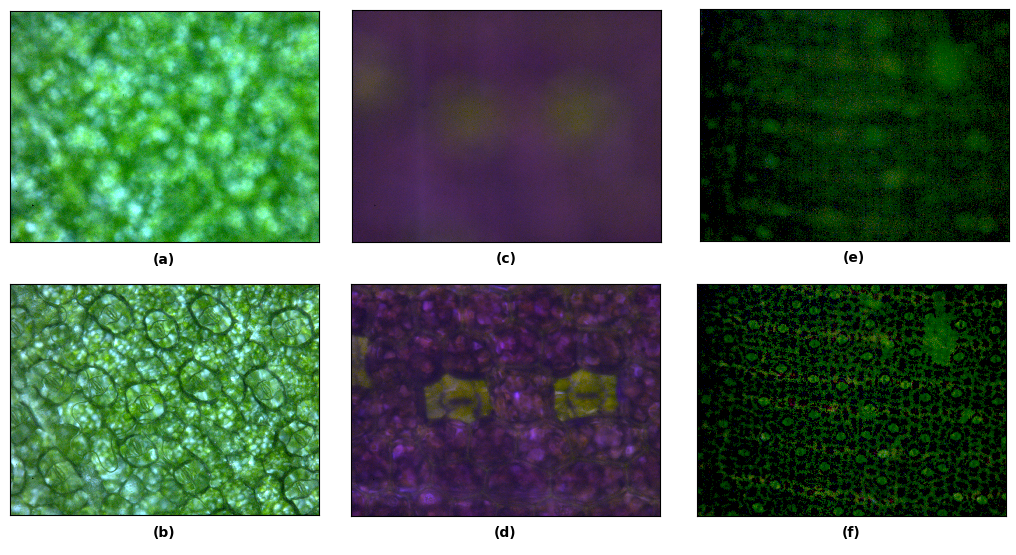
\includegraphics[scale=0.4]{images/datasets.png}
	\centering
	\fautor
\end{figure}

\subsection{Acquisition and Usage Protocols}

We will refer to the datasets as \textit{Callisia}, \textit{Tradescantia} and \textit{Cthenante} for notation simplicity. The \textit{Callisia} and \textit{Tradescantia} datasets were acquired with the z-stacking method in the SteREO Discovery.v20 microscope, whereas the \textit{Cthenante} dataset was acquired with the AxioLab A1 microscope. The workstation was connected to the microscopes by means of the ZEISS Axiovision version 4.8 software package. The z-stacks were manually built, i.e. the axial location of the objective was manually changed.

The SteREO Discovery.v20 microscope allows a precise measurement of the objective height, and the slices were acquired with a distance of 10 $\mu$m between each other - the maximum manually achievable distance. For both microscopes, the acquisition started with the objective height above the focal plane and, therefore, a completely blurred image. Then, the objective was progressively lowered in the $z$ axis, and at each step, an image was taken; this process was done until the objective height was below the focal plane and the images were blurred again.

The z-stacks were registered for image fusion after the eligible images in each set were chosen. Therefore, after the IQA method was applied, each set of eligible images was aligned with the TrakEM2 package, an ImageJ-based tool for processing and analyzing microscopy images. It includes methods for lens distortion correction, stitching, serial section alignment, correction of section thickness, and contrast adjustment \cite{saalfeld2019computational}. TrakEM2 uses  a particular combination of methods. The feature extraction was done with a custom implementation of the \sigla{SIFT}{Scale Invariant Feature Transform}, together with a custom extension of the \sigla{RANSAC}{Random Sample Consensus} method for parameter estimation and the geometric consensus filtering process with the expected transformation model and a maximal expected error as parameters \cite{saalfeld2019computational}. 

Primarily, a subjective quality index based on the Mean Opinion Score (MOS) was built in order to validate the results. The mean opinion score is the average of values on a predefined scale that an observer assigns to his opinion about the performance of a system (in this case, the imaging system) across a sample of observers \cite{liu2019comprehensive}. Practically, it consists of integer numbers in the interval $[1,5]$ where 1 is the worst score and 5 is the best. With the output of three people - two microscopy experts and one from a non-microscopy field - a subjective index was created. Most of the images were classified as 1 and the maximum score was 3. The images were then labeled as 3 - \emph{eligible} and 1 or 2 - \emph{negligible} for the fusion process, respectively. The axial nature of the acquisition allowed for a contiguous set of eligible images in each dataset. \autoref{tab:dataset_info} presents some relevant properties of each dataset.

\begin{table}[ht]
    \centering
    \caption{Information about the proposed datasets.}
    \label{tab:dataset_info}
    \begin{tabular}{lccc}
        \toprule
        \textbf{Dataset} & \textbf{\textit{Callisia}} &
        \textbf{\textit{Tradescantia}} &
        \textbf{\textit{Cthenante}}\\
        \midrule
        \textit{Magnification} & 50x & 200x & 100x\\
        \textit{Step} & 10$\mu$m & 10$\mu$m & 4$\mu$m\\
        \textit{Number of images} & 56 & 66 & 55\\
        \textit{Eligible} & 9 & 2 & 16\\
        \textit{Sharp sequence} & 41 - 49 & 50 - 51 & 30 - 45\\
        \bottomrule
    \end{tabular}
    \centering
    \fautor
\end{table}

In order to use the proposed datasets for evaluation of new methods, it is necessary to take into account that several images are totally blurred, and an image quality assessment algorithm should yield a low metric number for such images. As the $z$ position approaches the optimal focal plane, the metric may start to produce better values. The images are named with the step of the $z$-stack starting at 1, so that the eligible images are easily located. The metric should yield the highest quality values are among the range of eligible images, depicted as 
``Sharp sequence'' in \autoref{tab:dataset_info}. When the axial position is not exceeds the limits of the sharp sequence, the metric values should decay. The datasets are capable of assessing the monotonicity, accuracy and precision of image quality metrics.

\section{Benchmark datasets}

Benchmark datasets are fundamental in computer vision and image processing research in order to track the performance, accuracy and efficiency of new methods and algorithms. The image quality assessment was also evaluated against literature methods with the well-known Computational and Subjective Image Quality database (CSIQ) image quality assessment database \cite{larson2010most} and the KonIQ database, the largest image quality assessment database to date \cite{hosu2020koniq}. 

The CSIQ database contains 30 original images of dimensions $512 \times 512$. Each image is distorted in four to five different levels separately by JPEG and JPEG-2000 compression, Gaussian blurring, global contrast decrements and additive pink Gaussian noise. The Gaussian blur subset with 150 images was employed in the proposed analysis. The dataset also contains 5000 subjective rates done by 35 different observers, By means of a MOS index. 

The KonIQ database was built in order to evaluate the performance of a deep learning method for blind image quality assessment. It consists of 10073 images of dimensions $1024 \times 768$ with different labels for brightness, contrast, colorfulness and sharpness. The labels were generated from 1.2 million MOS rating of 1459 observers. One dissimilar feature of KonIQ when compared to CSIQ is that the quality assessment should be done among different scenes with different levels of degradation. \autoref{fig:csiq_example} shows two samples of the CSIQ database, and \autoref{fig:koniq_example} presents both blurred and sharp samples from the KonIQ image.

\begin{figure}[htb]
    \centering
    \caption{Samples from the CSIQ database: blurred image (a) and sharp image (b).}
    \label{fig:csiq_example}
    \begin{subfigure}[t]{0.45\textwidth}
        \centering
        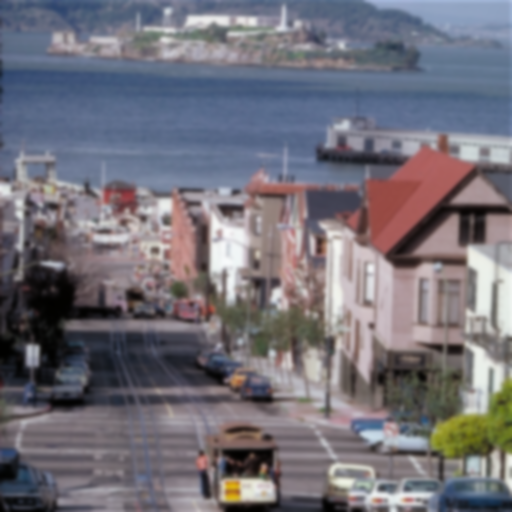
\includegraphics[height=5cm]{images/csiq_blurred.png}
        \caption{}
    \end{subfigure}%
    ~ 
    \begin{subfigure}[t]{0.5\textwidth}
        \centering
        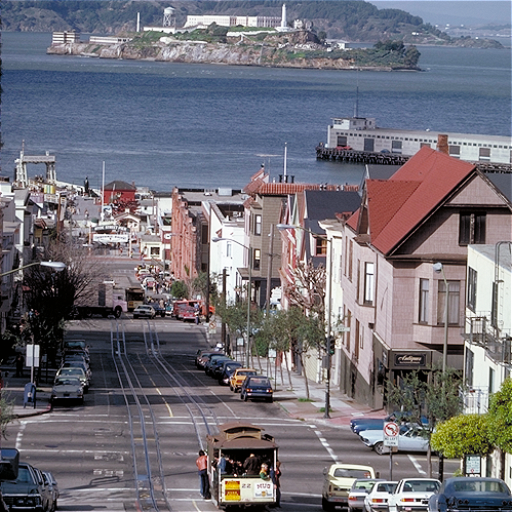
\includegraphics[height=5cm]{images/csiq_sharp.png}
        \caption{}
    \end{subfigure}
    \centering
    \fdireta{larson2010most}
\end{figure}

\begin{figure}[htb]
    \centering
    \caption{Samples from the KonIQ database: blurred image (a) and sharp image (b).}
    \label{fig:koniq_example}
    \begin{subfigure}[t]{0.45\textwidth}
        \centering
        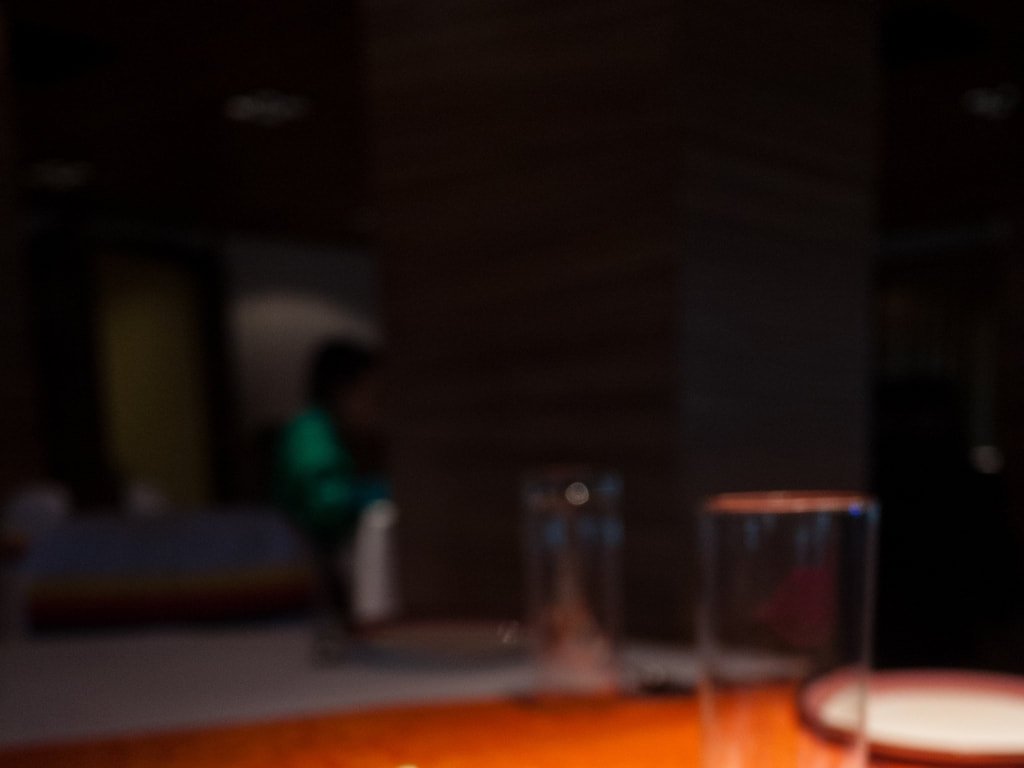
\includegraphics[height=4cm]{images/koniq-blurred.jpg}
        \caption{}
    \end{subfigure}%
    ~ 
    \begin{subfigure}[t]{0.45\textwidth}
        \centering
        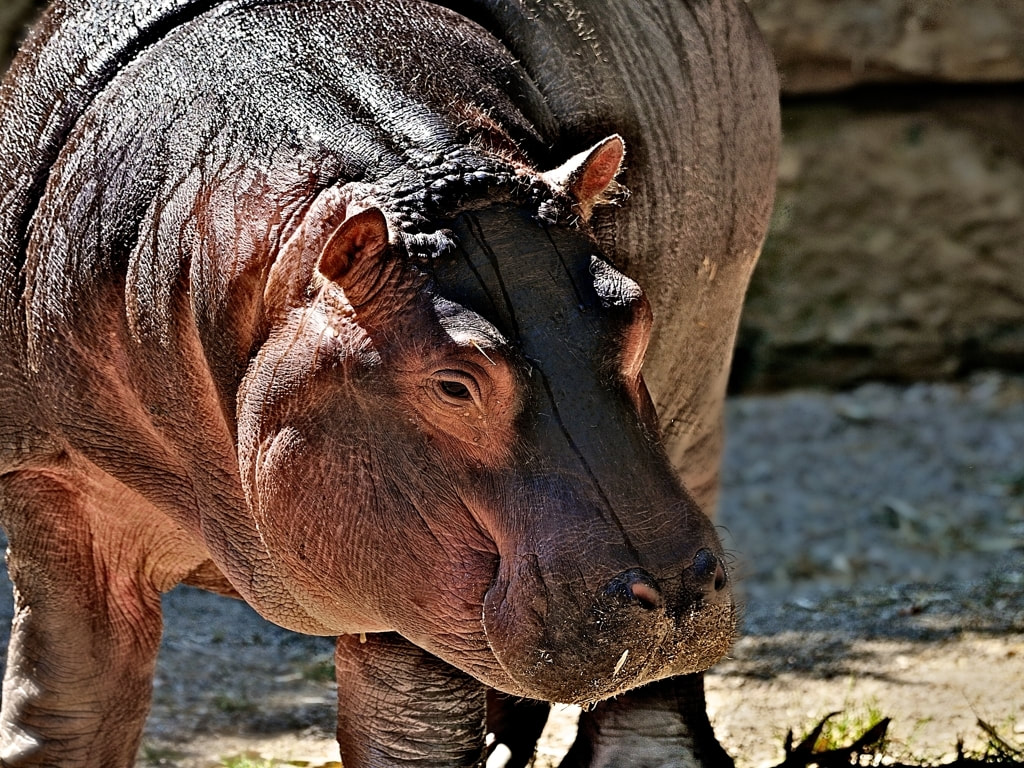
\includegraphics[height=4cm]{images/koniq-sharp.jpg}
        \caption{}
    \end{subfigure}
    \centering
    \fdireta{hosu2020koniq}
\end{figure}

\section{NR-IQA in Bright-field Microscopy Images Using the Fourier Transform and Kurtosis}
The next step is to devise a quantitative representation of sharpness for each image in each dataset. This measure allows for the selection of the eligible images through statistical analysis and the posterior registration of the selected slices. We propose a new method for image quality assessment based on a sampling process of the Fourier spectrum and posterior analysis of the coefficients as a probability distribution using summary and descriptive statistics. This section presents each stage of the method: pre-processing, Fourier spectrum sampling and statistical analysis. Figure \ref{fig:pipeline} shows a diagram of the proposed method.

\begin{figure}[ht]
  \centering
  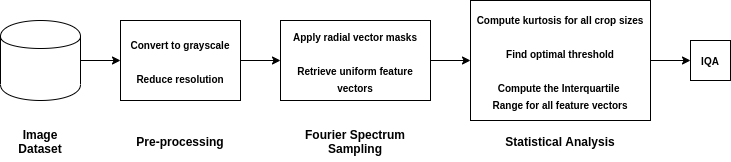
\includegraphics[scale=0.6]{images/nr-iqa_pipeline.png}
  \caption{Pipeline of processing steps of the propose no-reference IQA method.}
  \label{fig:pipeline}
\end{figure}

First, the image undergoes a grayscale conversion with the luminance method \cite{ponti2016image} - a 
linear combination of the three channels of a RGB image, as shown in the matrix equation given by

\begin{equation}
    \label{eqn:luminance}
    I_{luminance} = 0.299R + 0.587G + 0.114B,
\end{equation}

\noindent where $I_{luminance}$ is the matrix that represents the grayscale converted image, $R$, $G$ and $B$ represent the matrices of the red, green and blue channels, respectively. Next, the resolution of each grayscale image is reduced by half, from 2560 $\times$ 1920 to 1280 $\times$ 960. This provides shorter computational times. We empirically observed that  reduction in resolution did not compromise the results. We employed a bilinear interpolation that uses the four nearest neighbors to estimate the intensity at a given location \cite{gonzalez2018digital}, described as

\begin{equation}
\label{eqn:bilinear_interpolation}
I_{resized}(x,y) = ax + by + cxy + d.
\end{equation}

The CLAHE algorithm is then applied  to deliver a more uniform image to the Fourier Transform. This is necessary as microscopy images are influenced by illumination conditions, the focus adjustment itself and also physical properties of the transmitted or reflected light.

Next, the DFT is applied to all images and the resulting spectra are analyzed. The Fourier spectrum of a two-dimensional signal such as an image is a matrix with complex coefficients and zeros on each of its four corners and carries information about frequency bands of the image, characterized as a distribution. Our approach requires a shift between the first and third quadrants, and also the second and the fourth quadrants, to the center of the matrix. The unshifted and shifted Fourier spectrum of an grayscale airplane test image are shown in Figures \ref{fig:fourier_spectrum}.(c) and \ref{fig:fourier_spectrum}.(d), respectively. 

\begin{figure}[ht]
	\centering
	\caption{Original image \textbf{(a)}, luminance grayscale converted image \textbf{(b)}, unshifted Fourier spectrum of the grayscale image \textbf{(c)}, shifted Fourier spectrum of the grayscale image \textbf{(d)} and frequency bands as rings of radius $\{r_{i}: i\in\mathbb{N}^{*}\}$ drawn over the 2D spectrum \textbf{(e)}.}
	\label{fig:fourier_spectrum}
	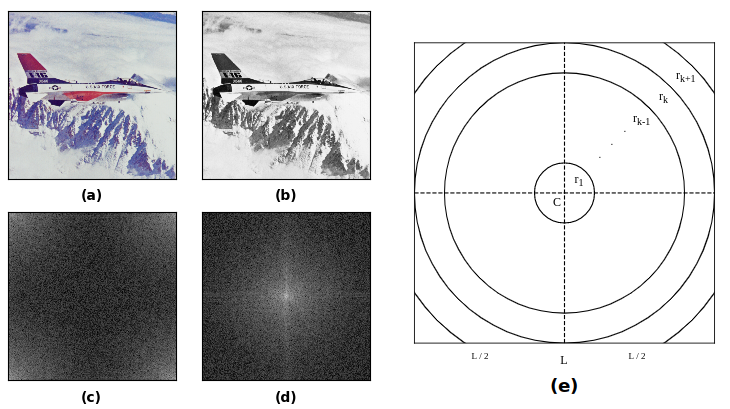
\includegraphics[scale=0.6]{images/fourier_spectrum.png}
	\centering
	\fautor
\end{figure}

The frequency information may be retrieved from the shifted Fourier spectrum by means of concentric circles drawn over it in the form of masks. Theoretically, the number of masks that may be applied to the spectra is infinite, but the discrete nature of images renders a finite number of masks. Let the matrix of DFT coefficients be graphically represented in Figure~\ref{fig:fourier_spectrum}.(e) and be mathematically denoted as a square of side $L = \max{(m,n)}$, $k = L / 2$ be the maximum radius value for circles within the square and $C = (k,k)$ be the center of the infinite set of concentric circles inscribed in the square. Circles with small radii comprise low-frequency information whereas large radii values cover high-frequency coefficients.

Taking into account the pixel resolution of the input images, it makes sense to sample the information, otherwise, the computational complexity and running times of the algorithm for one image alone would be impractical. Moreover, it is also unrealistic to evaluate every area under each concentric circle to retrieve the frequency content of an image; there is also no standard discrete amount of frequency bands to be evaluated.

Therefore, we drove our efforts to comprise as much information about each frequency band as possible and explored the fact that the Fourier spectrum of a real function such as an image is even, i.e. symmetric concerning its origin. Instead of the pure complex coefficients, we represent the Fourier spectrum by the magnitude of its coefficients, given by

\begin{equation}
\label{eqn:magnitude_of_DFT}
K(m,n) = 
    \log_{e}{\left(1
    + \sqrt{
        [\operatorname{Re}{(\hat{g}(m,n))}]^{2}
        + [\operatorname{Im}{(\hat{g}(m,n))}]^{2}
      }
    \right)},
\end{equation}

\noindent where $\hat{g}(m,n)$ are the complex Fourier coefficients of an image $g(x,y)$. We propose to sample the spectrum by means of radial lines as masks, i.e. white antialiased lines are drawn over a zero-valued matrix of dimensions 1280 $\times$ 960, the same dimensions of the Fourier spectrum of the reduced image, which are then element-wise multiplied by the spectrum. The lines are created from the $(x_{c},y_{c})$ center of the spectrum to points in an approximate radial position, which is calculated by

\begin{equation}
\label{eqn:points_on_radii}
P(x,y) = 
    (
    x_{c} r_{j} \cos{a_{j}}, 
    y_{c} r_{j} \sin{a_{j}}
    )
\end{equation}

\noindent with the set of angles $\{a_{j}\}$ in the radian form, computed as

\begin{align}
\label{eqn:angles}
\left\{
a_{j} : a_{j} = 
\frac{j \pi}{180}
\right\}
&&  j = \{0,5,...,100\}.
\end{align}

Equation
\ref{eqn:points_on_radii} is a
floating-point ordered pair, rounded to the nearest integer value in order to represent a location in the spectrum. The
antialiased lines are drawn with a Gaussian filtering process. After all the lines have been generated, the mask is similar to what is shown in Figure~\ref{fig:radial_masks}:

\begin{figure}[ht]
	\centering
	\caption{Final mask of antialised radial lines to sample the Fourier spectrum.}
	\label{fig:radial_masks}
	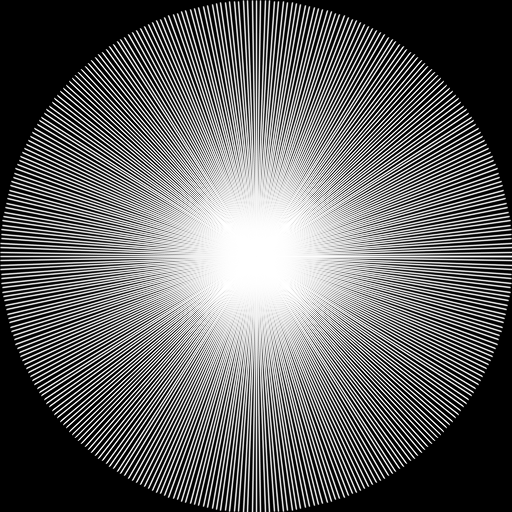
\includegraphics[scale=0.5]{images/radial_masks.png}
	\centering
	\fautor
\end{figure}

The extraction of the region of interest from the spectrum with the mask of radial lines results in arrays of complex coefficients that represent samples of the frequency profile of the image. However, despite the antialiasing, the resulting arrays differ in length since the original data is discrete. The vectors go through an element-wise average, which results in a one-dimensional vector as a descriptor of the frequency spectrum, and before such average, we find the smallest vector size among all of them and discard the remaining information in all of them. For comparison purposes, a square image of side $L$ yields a feature vector of size $1 / 2L$.

Next, the sharpness information of the image is encoded into a low-dimensional and concise representation that may undergo analysis with statistical tools and the mathematical properties of the Fourier spectrum. The feature vectors from each image need to be transformed into a model that is suitable for techniques such as Descriptive Statistics or Bayesian Inference, and therefore must be mapped onto the probability space $\Omega = [0,1]$. Hence, we apply an operator $T : \ell^{2}(\mathbb{Z}^{2}) \rightarrow \ell^{2}(\mathbb{Z}^{2})$, written as

\begin{align}
\label{eqn:probability_operator}
T(x_{i}) = \frac{x_{i}}{\sum_{j=0}^{n-1}x_{j}}
&&  i = \{0,1,...,n-1\},
\end{align}

\noindent where each $x_{i}$ is a value of the descriptor which will be mapped onto a probability. Note that each feature vector after the sampling process is a distribution in the scope of the Distribution Theory, i.e. a continuous linear functional defined on a space of smooth (functions with continuous derivatives up to some desired order over some domain \cite{weisstein2020smooth}) and compact supported (the functions yields zero outside of a closed and bounded set \cite{weisstein2020compact}) functions, with values in the range $[0,\infty)$. Therefore, it makes sense to apply the operator that maps it to a probability. This proposition was proved in \autoref{chapter:definitions-and-proofs}, which summarizes several definitions from Mathematical Analysis, Measure Theory and Distribution Theory required for the proof.

Information embedded in the low-frequency components of each feature vector corresponds to the Dirac delta distribution within the PSF of the microscope and should be discarded since it is equal to all images and does not resemble blur information; the removal should be done with caution so that the remaining information is enough to represent the blur profile of the image and allow the further selection by the image quality metric. An optimal threshold should be calculated for ``cropping'' the data, i.e. only a subset of it will represent the sharpness information. The threshold is chosen to maximize the difference between the maximum and the minimum among a set of kurtosis values of each feature vector.

The array of kurtosis for every crop size is computed as follows. The crop size initializes as zero and is used to compute the kurtosis of the entire set $\{x_{1},x_{2},...,x_{n}\}$ of all descriptors. The crop size is then incremented by 1, yielding the subset $\{x_{2},x_{3},...,x_{n}\}$. This process is done until the kurtosis for all crop sizes of the feature vectors is computed. Algorithm \ref{alg:kurtosis_array} summarizes the computation of kurtosis for all crop sizes:

\begin{algorithm}[H]
	\caption{Kurtosis computation}
	\label{alg:kurtosis_array}
	\begin{algorithmic}[1]
	    \State // $X_{c \times n}$: dataset of $n$ descriptors with size $c \in C$, where \\ // $C = \{0,1,...,size(descriptor)\}$ 
	    
	    \\
	    
	    \State // $T(X)$: operator from equation \ref{eqn:probability_operator} to map the \\ // descriptors onto probability distributions
	   
        \\
        
		\State $X \gets T(X)$
		\State $A \gets zeros(c, n)$
		
		\For {\textbf{each} crop size $c$ in $C$}
		    \For{\textbf{each} descriptor $i$ in $\{1,2,...,n\}$}
		
        		\State $A[crop][i] \gets$ \textbf{kurtosis}$\left(X[i].subset(0, crop)\right)$
		
		    \EndFor
		\EndFor
		
		\\
		
		\Return $A$
	\end{algorithmic}
\end{algorithm}

\noindent Next, the optimal threshold computation is done with algorithm~\ref{alg:cut_threshold}. It aims to produce a crop size to maximize the peak to peak value, i.e. the difference between the maximum and minimum values in the dataset. This allows low-frequency information to be discarded from the PSF without loss of the blur.

\begin{algorithm}[ht]
	\caption{Find the optimal dataset variability threshold}
	\label{alg:cut_threshold}
	\begin{algorithmic}[1]
 		\State // $A_{c \times n}$: matrix with kurtosis values for all $n$ descriptors that were computed at every crop \\ // size $c \in C$, where \\ // $C = \{0,1,...,size(descriptor)\}$ 
		
		\\
		
		\State $threshold \gets 0$
		\State $maximum \gets \infty$
		\For {\textbf{each} crop size $c$ in $C$}
		\State $row \gets \{A_{c,1},A_{c,2},...,A_{c,n}\}$ 
		
		\State $a \gets$ \textbf{max}$(row)$
		
		\State $b \gets$ \textbf{min}$(row)$
		
		\\
		
		\If{$a < 0$ or $b < 0$}
		    \State \textbf{continue}
		\EndIf
		
		\\
		
		\State $range \gets a - b$
		
		\\
		
		\If{$range > maximum$}
		    \State $maximum \gets range$
		    \State $threshold \gets c$
		\EndIf
		
		\EndFor
		\\
		\Return $threshold$
% 		\EndFunction
	\end{algorithmic}
\end{algorithm}

The low-frequency is discarded in each feature vector up to the optimal threshold, and the IQR measure is computed for all of them. In this work, the IQR value of the feature vector of an image corresponds to the amount of details, i.e. high-frequency content on it: the higher the IQR value, the sharper the image is. Finally, an estimate of the subset of images that is eligible for the fusion process is then obtained by the $z$-score transformation by choosing the images that locate at one or more standard deviation units away from the mean.

\section{Laplacian of Gaussian-based Multi-focus Bright-field Microscopy Image Fusion}
The NR-IQA method provided a sharpness measure for each image of the datasets and such numerical representations were analyzed with the $z$-score; at this point, the estimate of eligible images was prompted to the user and the real eligible ones were chosen. The obtained subset is registered by means of the SIFT-based z-stack alignment tool of the TrakEM2 package. The subsequent stage is to perform the fusion of images in the before-mentioned subset. We propose a multi-focus bright-field microscopy image fusion algorithm with the Laplacian of Gaussian edge detection filter and the energy of edges. Fig.~\ref{fig:fusion_pipeline} shows a diagram of the proposed method.

\begin{figure}[ht]
    \centering
    \caption{Diagram of the proposed multi-focus bright-field microscopy image fusion algorithm.}
    \label{fig:fusion_pipeline}
    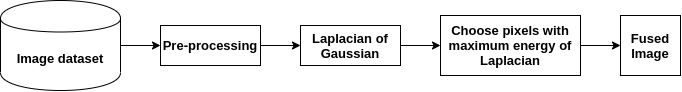
\includegraphics[scale=0.65]{images/fusion_pipeline.png}
    \centering
    \fautor
\end{figure}

The grayscale version of the selected images is again used for fusion; since the images were converted with the luminance method, the edges are preserved and therefore the edge detection may be successful. Other methods from the \emph{Luminance} family, e.g. \emph{Luminance}, \emph{Luminance\'}, \emph{Luma} and \emph{Decolorize}, are also suitable \cite{kanan2012color}.

The images then undergo the Laplacian of Gaussian filter - a spatial filtering algorithm that extracts edges of a smoothed image. The Laplacian is a second-order derivative isotropic linear operator, based on the Laplacian of a function, which defines an edge as the zero-crossing of the second derivative of a function. First and foremost, the Laplacian of a function is denoted by

\begin{equation}
\label{eqn:laplacian_of_function}
\nabla^{2}g(x,y) = \frac{\partial^{2} g(x,y)}{\partial x^{2}}
                    +
                  \frac{\partial^{2} g(x,y)}{\partial y^{2}},
\end{equation}

\noindent where $g(x,y)$ is the input image. For the discrete case (which applies to the digital images), the Laplacian operator is achieved by means of a convolution. The approximation of the second derivatives in each dimension yields the following convolution kernel

\begin{equation*}
\label{eqn:discrete_laplacian}
\begin{bmatrix}
0 & 1 & 0 \\
1 & -4 & 1 \\
0 & 1 & 0
\end{bmatrix}.
\end{equation*}

Similarly, instead of extracting edges with the Laplacian filter only, the Laplacian of Gaussian filter performs a Gaussian filtering process to remove noise and smooth the images before retrieving the edges \cite{marr1980theory}. This approach applies to cases where the quality and reliability of edges obtained by the Laplacian operator are sensitive to noise, and also plays the role of distinguishing the blurry regions from the sharp ones in our approach; pixels belonging to sharp regions will suffer a stronger smoothing effect in comparison to blurry pixels. For our application, an image is convolved with a two-dimensional Gaussian filter, denoted by

\begin{equation}
\label{eqn:gaussian_filter}
S(x,y) = g(x,y) \ast \frac{1}{\sqrt{2 \pi \sigma}} e^{- \frac{x^{2} + y^{2}}{\sigma^{2}}},
\end{equation}

\noindent where $S(x,y)$ is the smoothed version of the image, $g(x,y)$ is the input image and $\sigma$ is the standard deviation of the Gaussian function. Then, the Laplacian is applied to the smoothed image $S$. Both operators are linear and shift-invariant and therefore can be applied in any order, but the Gaussian filter is commonly applied first if the application required separated filters. In our case, the Laplacian of Gaussian operator can be defined as

\begin{equation}
\label{eqn:laplacian_of_gaussian}
LoG(x,y) = - \frac{1}{\pi \sigma^{4}}
            \left[
                1 - \frac{(x^{2} + y^{2})}{2 \sigma^{2}}
            \right]
            e^{- \frac{x^{2} + y^{2}}{2 \sigma^{2}}}.
\end{equation}

\noindent The $\sigma$ parameter is responsible for the smoothing magnitude. The convolution kernel is then a combination of both Laplacian and Gaussian filters; higher $\sigma$ values increase the effective kernel size consequently the smoothing effect. The next step is to retrieve the energy for each region, also based on the fact that blurry regions of an image present less high-frequency components than sharp regions. This stems from the fact that sharp regions are prone to have more edges than smoothed ones, hence a higher energy level. The higher the number the edges in an area of the image, the better the focus on it. Therefore, pixels that correspond to edges are chosen to form the fused image. Their spatial location is used to construct an RGB image by retrieving the content of the three channels from those pixels and assigning them to the final image.